\documentclass[a4paper, 12pt]{article}

\usepackage{listings}
\usepackage{color}

\definecolor{dkgreen}{rgb}{0,0.6,0}
\definecolor{gray}{rgb}{0.5,0.5,0.5}
\definecolor{mauve}{rgb}{0.58,0,0.82}

\lstset{frame=tb,
	language=C,
	aboveskip=3mm,
	belowskip=3mm,
	showstringspaces=false,
	columns=flexible,
	basicstyle={\small\ttfamily},
	numbers=none,
	numberstyle=\tiny\color{gray},
	keywordstyle=\color{blue},
	commentstyle=\color{dkgreen},
	stringstyle=\color{mauve},
	breaklines=true,
	breakatwhitespace=true,
	tabsize=3
}

\usepackage[english]{babel}
\usepackage{microtype}
\usepackage{graphicx}
\usepackage{amsmath}
\usepackage{index}

\makeindex

\begin{document}
	\title{Tutorat microprocesseur}
	\author{Corentin GIELEN, Florian DERLIQUE, Miaoqi WANG, Maxence NEUS}
	\maketitle
	
	\newpage
	\tableofcontents
	\newpage
	
	\section{Introducion}
		Nous avons à réaliser un radar de contrôle routier.
		Le radar doit pouvoir réaliser les fonctions suivantes :
		\begin{enumerate}
			\item Mesurer la vitesse d'un véhicule qui entre dans sa zone d'action
			\item Permettre de changer la vitesse maximale autorisée à l'aide d'un clavier
			\item Nous avons aussi ajouté des afficheurs 7 segments pour afficher la vitesse alors qu'elle est tapée.
			\item Si la vitesse mesurée est supérieure à la vitesse maximale, activer le flash et envoyer la vitesse mesurée sur l'imprimante série
		\end{enumerate}
	
		On nous demande ici en plus, de ne flasher que lorsque le vehicule se trouve à une distance de moins de 30m du radar afin que l'appareil photo puisse avoir une bonne vue de la plaque d'immatriculation. Cette restriction nous as posé quelque problème que nous detailliron plus tard dans la partie sur les limites du système.
		
		
	\newpage
	\section{Architecture Matérielle}
		\subsection{Matériel}
		Nous avons à notre dispositon les éléments suivants :
		\begin{itemize}
			\item Un télémetre qui fournit un signal analogique proportionnel à la distance entre le radar et la voiture
			qui donne une valeur entre 0V pour une distance de 0m et 5v pour une distance de 100m
			\item Un détecteur de présence qui passe de l'état 0 à l'état 1 lorsqu'une voiture entre dans le champ de mesure du télémetre
			\item Un flash que l'on peut déclancher directement sur un pin digital
			\item Une imprimante série pour imprimer les vitesses mesurées
			\item Les composants standards
		\end{itemize}	
		\subsection{Mise en place de l'architecture}
		\begin{figure}[h]
		\centering
		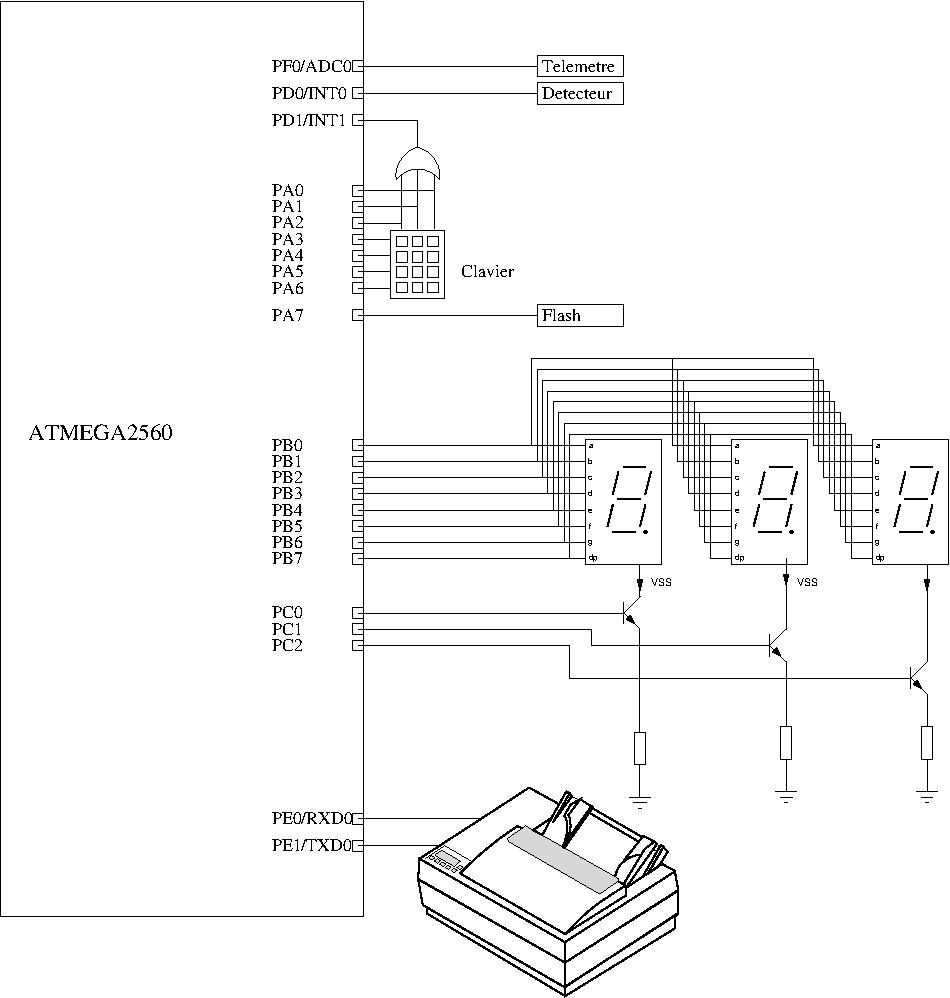
\includegraphics[width = 9cm]{schema.jpg}
		\caption{schema de cablage}
		\end{figure}
		\newpage
		\subsubsection{Interface utilisateur}
		Pour réaliser la fonction 2, nous avons besoin de permettre à l'utilisateur de rentrer une nouvelle valeur pour la vitesse maximale authorisée. Pour ce faire, nous avons incorporer un clavier 12 touches (0-9, Valider, Annuler) et 3 afficheurs 7 segments multiplexés pour afficher la valeur entrée à l'utilisateur.\\
		Le clavier est branché sur les pins PA[0:6] avec une porte OU qui permettra par la broche PD1/INT1 de travailler par interruption pour la lecture du clavier.\\
		Pour ce qui est des afficheurs 7 segments, ils sont reliés au port B pour la valeur à afficher et multiplexé par les pins PC[0:2] qui font la conection des bases des afficheurs à la masse via des transistors et des résistances de tirage.
		\subsubsection{Appareils de mesure}
		Comme le Télémetre nous fournis une valeur analogique, nous avons choisis de le relier à la broche PF0/ADC0 pour pouvoir réaliser une conversion dessus.\\
		Nous avons choisis d'utiliser le détecteur de présence par intéruption, nous le relions donc à la broche PD0/INT0.\\
		\subsubsection{Sorties utilisateur}
		Pour le flash, nous l'avons relié à la dernière broche inutilisée du port A, PA7, nous supposons qu'un appareil photo déclanchable par un front montant est relié à la même broche pour pouvoir prendre une photo de l'automobiliste qui est en exces de vitesse.\\
		L'impimante série est reliée à l'interface USART0 (PE0/RXD0;PE1/TXD1), L'imprimante fonctionne à 1200 bauds, 8bits de message, 1 bit stop et pas de parité, son initialisation sera développée dans la section 3.\\
	\newpage
	\section{Architecture Code}
		\subsection{Première approche}
		Nous avons commencé par réaliser une escisse de code en pseudo code afin de mettre en place
		\begin{lstlisting}
			Init:
			
			int Pos1;
			int Pos2;
			int cpt_mersure = 0;
			int clavier[ ];
			int vitesse_limite;
			int touche;
			int cpt_clavier=0;
			int affiche[]
			
			Loop:
			sleep;
			jmp loop;
			
			IRQ_Detecteur:
			if PDO==1
			int watch_dog a 0,5s (a 1s si quelqu un roule a plus de 220 km il ne serait pas forcement flashe)
			else	
			reinistialisation watch_dog
			RETI
			
			IRQ_WDT:
			activer la convertion d une valeur 
			RETI
			
			IRQ_CONVERTION: (quand convertion fini)
			if cpt_mersure == 0
			Pos1= mesure
			cptm = 1
			if cpt_mesure==1
			Pos2=mesure
			if (Pos1-Pos2) > vitesse limite et Pos2 < 30 
			flash
			envoie de la valeur sur le port serie 
			cptm == 0
			RETI	
			
			IRQ_CLAVIER:
			touche = clavier[touche_appuier]
			
			if touche == V
			RETI
			else if touche == C
			Vitesse_limite=0				
			else if cpt==0
			Vitesse_limite=touche
			call afficheur
			cpt++
			else if cpt==1
			Vitesse_limite*=10
			Vitesse_limite+touche
			call afficheur
			cpt++
			else if cpt==2
			Vitesse_limite*=10
			Vitesse_limite+touche
			call afficheur
			cpt=0
			RETI
			
			Afficheur:
			affiche[2]=vitesse_limite%100	
			affiche[1]=(vitesse_limite/10)%10
			affiche[0]=vitesse_limite/100
		\end{lstlisting}
	
		\subsection{Initialisation}
		Le convertisseur analogique numérique (ADC) est mis en place de sorte qu'il réalise des convertions sur demande en lisant sur la broche PF0/ADC0 en envoyant une interuption à la fin de la convertion.
		\begin{lstlisting}
			//ADC (convertion ADC0, single convertion)
			ADMUX = 0b0110 0000
			ADCSRA = 0b1000 1111
			ADCSRB = 0x00
		\end{lstlisting}
		\newpage
		ADMUX:
		\begin{center}
		\begin{tabular}{|c|c|c|c|c|c|c|c|}
		\hline
		REFS1 & REFS0 & ADLAR & MUX4 & MUX3 & MUX2 & MUX1 & MUX0\\
		\hline
		0 & 1 & 1 & 0 & 0 & 0 & 0 & 0\\
		\hline
		\end{tabular}
		\end{center}
		\begin{itemize}
			\item[REFS[1:0]] : On prends la réference sur 5V.
			\item[ADLAR] : On choisis de ne lire que les bits de poids fort, on choisis donc d'aligner à gauche.
			\item[MUX[4:0]] : On fait la convertion sur ADC0, soit l'adresse MUX = 0 0000.
		\end{itemize}
		
		ADCSRA:
		\begin{center}
			\begin{tabular}{|c|c|c|c|c|c|c|c|}
				\hline
				ADEN & ADSC & ADATE & ADIF & ADIE & ADPS2 & ADPS1 & ADPS0\\
				\hline
				1 & 0 & 0 & 0 & 1 & 1 & 1 & 1\\
				\hline
			\end{tabular}
		\end{center}
		\begin{itemize}
			\item[ADEN] : On active l'ADC.
			\item[ADCS; ADATE; ADIF] : Utilisés lors de l'utilisation de l'ADC donc pas utiles pour l'initialisation, on laissera ici tout à 0 pour avoir l'ADC à la demande.
			\item[ADIE] : Interrupt Enable.
			\item[ADPS[2:0]] : Prescaler, on veut que l'ADC fonctionne entre $50\ kHz$ et $200\ kHz$, la clock de l'ATMEGA etant à $16\ Mhz$, une division par 128 nous donne une fréquence acceptable (soit ADPS[2:0] = 000)
		\end{itemize}
		ADCSRB: Pas de bits utiles pour nous.\\
		
		Nous utiliserons des interruptions pour le clavier et pour le détecteur.
		\begin{lstlisting}
			EIMSK@IO <- 0b00000011
			EICRA <- 0b00001101 
		\end{lstlisting}
		On active ici les interuptions sur INT1 et INT0, le clavier sur INT0 en mode front montant et le détecteur sur INT1 en mode front montant et descendant.\\
		
		Nous utiliserons un WatchDog pour temporiser nos mesures, celui çi est ici reglé pour envoyer des interuptions toute les 0.5s (Ce choix est discuté dans la partie limites).
		\begin{lstlisting}
			//Watchdog (interruptions toute les 0.5s)
			WDTCSR = 0x10 // enable change
			WDTCSR = 0b0101 0101
		\end{lstlisting}
		WDTCSR:
		\begin{center}
			\begin{tabular}{|c|c|c|c|c|c|c|c|}
				\hline
				WDIF & WDIE & WDP3 & WDCE & WDE & WDP2 & WDP1 & WDP0\\
				\hline
				0 & 1 & 0 & 0 & 0 & 1 & 0 & 1\\
				\hline
			\end{tabular}
		\end{center}
		\begin{itemize}
			\item[WDIF] : Interupt Flag, en lecture uniquement.
			\item[WDE; WDIE] = 01 - Interrupt mode.
			\item[WDP[3:0]] = 0101 - Timing de 0.5s.
		\end{itemize}

		Pour envoyer les mesures à l'imprimante nous devons utiliser la liaison série de l'ATMEGA comme décrit en 2.2.3, nous avons caculé la valeur de UBRR grâce à la formule donné dans la documentation $UBRR = \dfrac{f_{osc}}{16*BAUD} - 1$ qui nous donne UBRR = 832, soit 0x340 à répartir sur les registres UBRRL0 et UBRRH0.
		\begin{lstlisting}
			//printer (envoi uniquement, pas de verification, conforme au CDCF)
			UBRR (f = 16MHz) = 832
			UBRRH0 = 0x03
			UBRRL0 = 0x40
			
			UCSR0A = 0x00
			UCSR0B = 0b0000 1000
			UCSR0C = 0b0000 0110			
		\end{lstlisting}
		UCSR0A:
			Globalement que des pins en lecture, donc rien à changer ici.	
		UCSR0B:
		\begin{center}
			\begin{tabular}{|c|c|c|c|c|c|c|c|}
				\hline
				RXCIE & TXCIE & UDRIE & RXEN & TXEN & UCSZ2 & RXB8 & TXB8\\
				\hline
				0 & 0 & 0 & 0 & 1 & 0 & 0 & 0\\
				\hline
			\end{tabular}
		\end{center}
		\begin{itemize}
			\item[RXCIE; TXCIE; UDRIE] : Interrupts Enable, pas utilisés ici
			\item[RXEN; TXEN] : Recieve/ Transmit Enable, ici on active uniquement la transmission
			\item[UCSZ2; RXB8; TXB8] : Utiles uniquement en transmission 9 bits.
		\end{itemize}

		UCSR0C:
		\begin{center}
			\begin{tabular}{|c|c|c|c|c|c|c|c|}
				\hline
				UMSEL1 & UMSEL2 & UPM1 & UMP0 & USBS & UCSZ1 & UCSZ0 & UCPOL\\
				\hline
				0 & 0 & 0 & 0 & 0 & 1 & 1 & 0\\
				\hline
			\end{tabular}
		\end{center}
		\begin{itemize}
			\item[UMSEL 1:0] = 00 - Mode Asynchrone
			\item[UPM 1:0] = 00 - Pas de parité
			\item[USBS] = 0 - 1 bit Stop
			\item[UCSZ 1:0] = 11 - 8 bit de message
			\item[UCPOL] Clock parity - utiles uniquement en mode Synchrone
		\end{itemize}
	
		On règle ici les afficheurs et le clavier comme décrit en 2.2.1.
		\begin{lstlisting}
			//Clavier et afficheurs
			DDRA@IO <- 0x78
			DDRB@IO <- 0xFF	 
			DDRC@IO <- 0x07
		\end{lstlisting}

		On reprends ici les différents vecteurs d'interruptions utilisés ainsi que les noms des subsoutines associées.
		\begin{lstlisting}
			//vecteurs d'interuption
			.org 0x0002
				JMP IRQ_detecteur
			.org 0x0004
				JMP IRQ_clavier
			.org 0x0018
				JMP IRQ_Watchdog
			.org 0x003A
				JMP IRQ_convertion
		\end{lstlisting}
		\subsection{Structure globale}
		Afin de réaliser les mesures de vitesses, nous n'avons à notre disposition que la position du vehicule, nous allons donc avoir besoin de mesurer la distance entre le radar et le vehicule à un intervale régulier pour pouvoir par la suite calculer la vitesse. \\
		Le processus de mesure commence lorsque le vehicule entre dans la zone de mesure du télémetre et que le détecteur de présence envoie un signal d'interruption qui amène à l'appel de la procédure d'interruption $IRQ\_detecteur$.
		
		\begin{lstlisting}
			// detection d'une voiture par le detecteur de presence  
			IRQ_Detecteur:
				si cpt_detection==0 alors saut init_watch // si le capteur est en front montant on initialise le WatchDog
				//si non on reinitialise le WatchDog 
				WDTCSR<-0b00010000
				WDTCSR<-0b00000000
				cpt_detection <- 0 
				RETI
				init_watch: 
					WDTCSR<-0b00010000
					WDTCSR<-0b01001101
					cpt_detection=1
				RETI
		\end{lstlisting}
		Cette procédure a pour but de démarrer ou d'arreter le WatchDog selon si le vehicule qui a été détecté entrait ou sortait de la zone de mesure (l'interuption est règlée pour être déclanchée sur front montant comme déscendant), cette distinction est faite grâce à une variable $cpt\_detection$ qui est mise à 1 lorsqu'un vehicule est présent dans la zone et à 0 lorsque ce n'est plus le cas.\\
		
		Par la suite, le WatchDog va maintenant déclancher des interuptions toute les 0.5s sur la procédure $IRQ\_WatchDog$ comme defini lors de l'initialisation. Voyons maintenant ce que fait cette procédure:\\
		
		\begin{lstlisting}
			//interuption du watch_dog
			// quand le watch_dog est activer on active la prise de mesure
			IRQ_WDT :
				ADCSRA<-0b11001111
				RETI
		\end{lstlisting}
		Ici tout ce que fait la procédure c'est lancer une convertion sur ADC0 afin de mesurer la distance du radar au vehicule, lorsque cette mesure sera faite, le convertisseur analogique numérique lancera une interruption qui déclanchera la procédure $IRQ\_convertion$.\\

		\begin{lstlisting}
			IRQ_CONVERTION: 	;quand la distance a ete convertie en valeur numerique
			mesure <- ADCH
			si CptMesure == 0 alors saut cpt0 ;la premiere mesure de vitesse 
			si CptMesure == 1 alors saut cpt1 ;2 eme mesure de vitesse
			
			cpt0:
			Pos1<-mesure 		;alors on stocke la valeur mesure par la conversion entre 0 et 255
			CptMesure <- 1 
			RETI
			
			cpt1:
			pos2<-mesure
			si(Pos1-Pos2)>VitesseLimite saut distflash 	;si la vitesse et superieur a la limite et que la voiture est a plus de 30m du tel
			CptMesure <- 0
			RETI
		\end{lstlisting}
		Si la vitesse mesurée est supérieure à la vitesse limite, alors on mets l'ADC en free running mode pour attendre que le vehicule soit à porté, alors à ce moment seulement on lencera la suite de la procédure.\\
		Si ce n'est pas le cas la procédure s'arrête ici.\\
		
		\begin{lstlisting}
			distflash:  				;si la vitesse est superieur on attends que la distance au radar soit inferieur a 30m
			
			posflash<-pos2 
			ADCSRA<-0b11101111 		;on active la mesure en continue
			
			condition:
			si posflash<76 alors saut port_serie  	;76 en analogique soit 255/100*30 pour avoir les 30m
			
			Adcloop:
			si ADCSRA & 0x10 != 0x10 saut Adcloop 	; si la conversion est fini 
			posflash<-ADCH
			jmp condition 
			
			;liaison serie -----------------------------------------------
			
			portSerie:
			ADCSRA <- 0x00			;desactive la mesure en continue 
			PORTA@IO<-0x80 				;flash
			CptEmission <- 0
			mesure<- Pos2-Pos1
			
			imprime:
			si ( UCSR0A&0x20 != 0x20) alors saut imprime 	;si le buffer et pres a envoyer
			
			envoie:
			si CptEmission== 0 alors saut unit
			si CptEmission== 1 alors saut diz  
			si CptEmission==2 alors saut cent
			si CptEmission==3 alors saut entree
			
			unit:
			unite<- (mesure%100)*3.6		;le compilateur ne prend pas en compte les virgules flottantes
			UDR0<- unite%10 +48
			retenu<- mesure/10 			;retenu car peut etre sup a 9
			CptMesure<-1
			jmp imprime
			
			dizaine:
			
			unite<- ((mesure/10)%10)*3.6 + retenu
			UDR0<- unite%10 + 48
			retenu<- mesure/10
			CptMesure<-2
			jmp imprime
			
			cent:
			unite <- (mesure/100)*3.6 + retenu
			UDR0 <- unite%10 + 48
			retenu <- mesure/10
			CptMesure<-3
			jmp imprime
			
			entree:
			UDRO<-27
			CptMesure<-3
			RETI
		\end{lstlisting}
		Cette procédure a pour but global de prendre une première mesure de vitesse au début de la zone de mesure, et si cette mesure de vitesse est supérieure à la vitesse maximale autorisée, alors le convertisseur analogique numérique est lancé en free running mode et le radar flashera le vehicule lorsque la mesure de position sera inférieure à 30m on lance la procédure de flash et d'envoi de la vitesse mesurée à l'imprimante. Ce choix est expliqué plus en détail dans la partie 4.1.\\
		Cette vitesse est d'abord convertie en $km/h$ à partir de la mesure en $m/s$ qui est utilisée en interne et ensuite envoyée caractère par caractère à l'imprimante, cette transmission aurait pu être faite par interruption, mais cela aurait alourdi grandement le code, nous avons donc choisis de travailler par scrutation pour allèger le code, même si ce choix alonge la procédure d'interruption lors d'un flash, mais cette interruption ne devrait pas survenir assez souvent pour créer un problème.
		De plus on notera l'utilisation des nombres à virgules flottantes qui ne sont pas natifs du language assembleur mais on supposera qu'un compilateur pourrait gérer ce calcul.
		
		\subsection{Changement de la vitesse limite par l'utilisateur}
		La vitesse limite authorisée doit pouvoir être modifiée à tout moment par l'utilisateur à l'aide du clavier, nous afficherons également la saisie sur les 3 afficheurs durant la durée de la saisie et nous désactiverons les afficheurs lorsque la saisie a été validée car ils ne seront pas utiles lors d'une utilisation normale. Cette saisie sera stockée dans 3 variables (une pour chaque digit) ce qui facilitera la saisie et nottament la correction.
		\begin{lstlisting}
			IRQ_Clavier: ;si contact entre les pin
			
			init_clavier:
			i<-0
			changeVitesse<-1
			
			parcours_clavier: ;on parcours le clavier jusqu a trouver le bon 
			PORTA@IO<-codeClavier@ROM[i]
			touche <- PINA@IO
			si (touche == 0x44 ) alors saut REINITclavier ;C
			si (touche == 0x41 ) alors saut VALIDEclavier ;V
			si (touche == PORTA@IO)&&(CptAff!=3) alors saut sauvTouche
			;sinon on incremente i
			i <- i + 1 
			JMP parcours_clavier
			
			;partie pour l afficheur 
			
			sauvTouche: ;sauvegarde de la touche 
			NBtouche<- i
			si CptAff==0 alors NBu<-NBtouche
			si CptAff==1 alors NBd<-NBtouche
			si CptAff==2 alors NBc<-NBtouche
			CptAff<-CptAff+1
			PORTA@IO <- 0b01111000
			RETI
			
			VALIDEclavier:
			BuffVitesseLimite<-NBu
			BuffVitesseLimite<-BuffVitesseLimite+(NBd*10)
			BuffVitesseLimite<-BuffVitesseLimite+(NBc*100)
			si BuffVitesseLimite>918 alors BuffVitesseLimite<-918
			VitesseLimite<-BuffVitesseLimite/3.6
			
			REINITclavier:
			CptAff<-0
			NBtouche<-0 
			NBu<-0
			NBd<-0
			NBc<-0
			BuffVitesseLimite<-0
			changeVitesse<-0
			PORTA@IO <- 0b01111000
			PORTB@IO <- 0x00
			PORTC@IO <- 0x00
			RETI
		\end{lstlisting}
		On utilise ici également un buffer pour stocker la vitesse à entrer sur 2 Obtets affin d'eviter des problèmes d'overflow lorsque l'utilisateur tape sur le clavier (en effet rien ne l'empêche de taper 999). Par la suite, nous mettons en place une valeur maximale de cette vitesse limite du côté du code etant donné que la mesure sera faite en m/s, il n'est pas possible de rentrer une vitesse limite plus grande que $918\ km/h$, en effet cette vitesse représente $255\ m/s$ qui remplis un octet.
		
		\section{Limites}
		\subsection{Limite de l'utilisation du WatchDog à 0.5s}
		Comme nous l'avons dit en 3.1, le choix de l'intervalle entre les mesures à 0.5s entraîne des limites pour certaines vitesses qui peuvent passer à travers la zone de flash des 30m et donc dans certains cas éviter d'être flashé en roulant à une vitesse assez précise.\\
		Cette limite peut être quantifiée sous quelques conditions:
		\begin{itemize}
			\item La première mesure est faite à exactement 100m du radar.
			\item Chaque mesure qui suit est faite à exactement 0.5s d'intervalle.
			\item Chaque calcul de vitesse se fait sur deux mesures, desquelles la seconde doit se retrouver dans la zone des 30m pour être flashé
		\end{itemize}
		Dans ces conditions, un rapide script (en annexe) nous permet de déterminer les plages de vitesses qui ne pourrait pas être mesurées avec ce système, on obtient les plages suivantes :
		\begin{itemize}
			\item $[33.4;35]\ m/s$ soit $[120;126]\ km/h$
			\item $[50;69.9]\ m/s$ soit $[180;251]\ km/h$
			\item $[100.2;+\infty[\ m/s$ soit $[360.7;+\infty[\ km/h$
		\end{itemize}
		Comme on peut le constater, ces plages sont problématiques car parfaitement atteignable par un vehicule sur une autoroute (particulièrement les 2 premières). Notre solution pour palier à ce problème est celle implémentée en 3.2, l'attente en free running mode que le vehicule puisse être flashé fait que la seule façon d'éviter le radar serait de traverser la zone des 30m en moins de temps qu'il n'en faut à l'ATMEGA pour réaliser une convertion, ce qui fait que la vitesse minimale pour y parvenir devient bien trop élevée pour qu'un vehicule terrestre puisse l'atteindre.
	
		\subsection{Approximation numérique}
		Par soucis de précision, on stocke la vitesse maximale tout comme les mesures effectuées en m/s, avec les distances en metres ramenés de $[0;100]$ sur $[0;255]$ pour avoir toute la précision disponible sur 8 bits, cela nous donne une précision de $\dfrac{100}{255} = 0.39m$ soit une précision sur la vitesse de $\dfrac{0.39m}{0.5s} = 0.78m/s = 2.8 km/h$ ce qui est admissible. De plus cette approche nous permet d'avoir une vitesse maximale mesurable de $360km/h$ contre les 255 que peuvent acceuillir un octet, ce qui est acceptable étant donné la difficulté d'un vehicule terrestre à atteindre une telle vitesse.\\
		Cette limite n'est engendrée que par la valeur du WatchDog, ce qui implique qu'elle peut être négligée par un simple changement de code (pour mesurer des vitesses sur un circuit de course par exemple).
 		Par ailleur les multiplications et divisions par des nombres flottants amènent des imprécisions duent aux arrondis.
		
		\newpage
		\section{Annexe}
		\subsection{Code Global}
		\begin{lstlisting}
			;interuption
			.equ EIMSK           = 0x3D
			.equ EICRA           = 0x69
			
			;watch_dog
			.equ WDTCSR        = 0x60
			
			;convertion analogique 
			.equ ADMUX 	= 0x7C
			.equ ADCSRB = 0x7B
			.equ ADCSRA = 0X7A
			.equ ADCL 	= 0x78
			.equ ADCH 	= 0x79
			
			;clavier A
			.equ DDRA	= 0x01
			.equ PORTA	= 0x02
			.equ PINA	= 0x00
			
			;communication serie 
			.equ UCSR0A	= 0x00C0
			.equ UCSR0B         = 0x00C1
			.equ UCSR0C         = 0x00C2
			.equ UBRR0L        = 0x00C4
			.equ UBRR0H        = 0x00C5
			.equ UDR0            = 0x00C6
			
			.equ DDRB	= 0x04
			.equ PORTB	= 0x05
			.equ PINB	= 0x03
			.equ DDRC	= 0x07
			.equ PORTC	= 0x08
			.equ PINC	= 0x06
			
			.dseg
			
			.org 0x0200
			
			CptDetection: .BYTE 1
			CptMesure: .BYTE 1
			CptEmission: .BYTE 1
			Pos1: .BYTE 1
			Pos2: .BYTE 1
			PosMesure: .BYTE 1
			Posflash: .BYTE 1
			VitesseLimite: .BYTE 1
			unite: .BYTE 1
			retenu: .BYTE 1
			
			
			;clavier
			
			touche: .BYTE 1
			CptAff: .BYTE 1
			i: .BYTE 1
			NBu: .BYTE 1
			NBd: .BYTE 1
			NBc: .BYTE 1
			NBtouche: .BYTE 1
			BuffVitesseLimite: .BYTE 2
			changeVitesse: .BYTE 1
			
			
			;------------------------------------------------------------------------------------------
			.cseg
			
			;initalisation des interuption INT
			.org 0x0002
			jmp IRQ_Detecteur ;interruption du detecteur
			
			.org 0x0004
			jmp IRQ_Clavier ;interuption clavier
			
			.org 0x0018
			jmp IRQ_WDT ;interruption watch_dog
			
			.org 0x003A
			jmp IRQ_CONVERTION ;interuption conversion dispo
			
			.org 0x0080
			
			;Code pour afficher
			codeAff:
			.DB 0x7E,0x0C,0x37,0x1F,0x4D,0x5B,0x7B,0x0E,0x7F,0x5F
			
			;Code de test du clavier
			codeClavier:
			.DB 0x42,0x0C,0x0A,0x09,0x14,0x12,0x11,0x24,0x22,0x21,0x44,0x41
			;0x44 -> C et 0x41 -> V
			
			;------------------------------------------------------------------------------------------
			;debut programme
			init:
			CptMesure <- 0
			EIMSK@IO <- 0b00000011 	        ;activation de INT0 et INT1
			EICRA <- 0b00001101 	                     ;on met le detecteur en activation front montant et descendant 
			;et INT 1 en montant    
			ADMUX <- 0b01100000 	;selection ADC0
			ADCSRB <- 0x00 		       ;tjr a 0
			;le premier 01 REFS1:2 choisi car valeur entre 0V et 5V 
			;ADLAR a 1 car on prends les 8 peremiers bit 
			
			DDRA@IO <- 0x78 			      ;tout en sortie sauf 0,1,2
			DDRB@IO <- 0xFF	 
			DDRC@IO <- 0x07
			PORTA@IO <- 0b01111000 	      ;allumage des broche du clavier en attente de contact
			;IRQ_Detecteur
			CptDetection <- 0
			
			;clavier
			CptAff <- 0
			NBu <-0
			NBd <-0
			NBc <-0
			
			;init imprime
			UBBR0L <- 0b01000000 ;16Mhz BaudRate : 1200
			UBBR0H <- 0b00000011 ;16Mhz BaudRate : 1200
			USCR0A <- 0x00
			USCR0B <- 0b00001000 
			USCR0C <- 0b00000110  ; pas de parite  8bit
			SEI 
			;--------------------------------------------------------------------------------------------------
			
			
			Loop: 	;boucle principal afficheur 7seg multiplexe
			si changeVitesse!=0 alors saut afficheVitesseChange
			jmp loop;
			
			afficheVitesseChange:
			PORTC@IO<-0x04
			PORTB@IO<-codeAff@ROM[NBu]
			PORTC@IO<-0x02
			PORTB@IO<-codeAff@ROM[NBd]
			PORTC@IO<-0x01
			PORTB@IO<-codeAff@ROM[NBc]
			PORTC@IO<-0x00
			jmp loop;
			
			
			;-------------------------------------------------------------------------------------
			
			IRQ_Detecteur:                                                     ;detection d une voiture par le detecteur de presence  
			si CptDetection==0 alors saut initWatch             ;si le capteur est en front montant on initialise le watch__dog
			;si non on reinitialise le watch dog 
			WDTCSR <- 0b00010000                              ;debloquage du watchdog
			WDTCSR <- 0b00000000                              ;reinitialisation
			CptDetection <- 0 
			RETI
			
			initWatch: 
			WDTCSR<-0b00010000
			WDTCSR<-0b01000101
			CptDetection <- 1
			RETI
			;-------------------------------------------------------------------------------------
			
			;interuption du watch_dog
			;quand le watch_dog est activer on active la prise de mesure
			IRQ_WDT:
			si changeVitesse!=0 alors RETI ; si l utilisateur tape sur le clavier on stop les mesure des vehicules le RETI ici empeche toute la suite du programme  
			ADCSRA<-0b11001111
			;ADEN 1 turn on adc
			;ADSC 1 premiere demande de conversion
			;ADATE 0 = une comversion
			;ADIF 0 car flag de fin 
			;ADIE 1 autorise les interuption 
			;APS2 1 1 facteur de division 128 nous devons realiser une mesure entre
			;50khz et 200khz etant a 8MHz si on divise par 128 ->62.5khz soit compris
			;entre 50 et 200
			RETI
			
			IRQ_CONVERTION: 	;quand la distance a ete convertie en valeur numerique
			mesure <- ADCH
			si CptMesure == 0 alors saut cpt0 ;la premiere mesure de vitesse 
			si CptMesure == 1 alors saut cpt1 ;2 eme mesure de vitesse
			
			cpt0:
			Pos1<-mesure 		;alors on stocke la valeur mesure par la conversion entre 0 et 255
			CptMesure <- 1 
			RETI
			
			cpt1:
			pos2<-mesure
			si(Pos1-Pos2)>VitesseLimite saut distflash 	;si la vitesse et superieur a la limite et que la voiture est a plus de 30m du tel
			CptMesure <- 0
			RETI
			
			;flash ------------------------------------------
			
			distflash:  				;si la vitesse est superieur on attends que la distance au radar soit inferieur a 30m
			
			posflash<-pos2 
			ADCSRA<-0b11101111 		;on active la mesure en continue
			
			condition:
			si posflash<76 alors saut port_serie  	;76 en analogique soit 255/100*30 pour avoir les 30m
			
			Adcloop:
			si ADCSRA & 0x10 != 0x10 saut Adcloop 	; si la conversion est fini 
			posflash<-ADCH
			jmp condition 
			
			;liaison serie -----------------------------------------------
			
			portSerie:
			ADCSRA <- 0x00			;desactive la mesure en continue 
			PORTA@IO<-0x80 				;flash
			CptEmission <- 0
			mesure<- Pos2-Pos1
			
			imprime:
			si ( UCSR0A&0x20 != 0x20) alors saut imprime 	;si le buffer et pres a envoyer
			
			envoie:
			si CptEmission== 0 alors saut unit
			si CptEmission== 1 alors saut diz  
			si CptEmission==2 alors saut cent
			si CptEmission==3 alors saut entree
			
			unit:
			unite<- (mesure%100)*3.6		;le compilateur ne prend pas en compte les virgules flottantes
			UDR0<- unite%10 +48
			retenu<- mesure/10 			;retenu car peut etre sup a 9
			CptMesure<-1
			jmp imprime
			
			dizaine:
			
			unite<- ((mesure/10)%10)*3.6 + retenu
			UDR0<- unite%10 + 48
			retenu<- mesure/10
			CptMesure<-2
			jmp imprime
			
			cent:
			unite <- (mesure/100)*3.6 + retenu
			UDR0 <- unite%10 + 48
			retenu <- mesure/10
			CptMesure<-3
			jmp imprime
			
			entree:
			UDRO<-27
			CptMesure<-3
			RETI
			
			;clavier ----------------------------------------------------------------------------------------------------
			
			;on considere un clavier comme en TP  avec *=C #=C
			;clavier
			
			IRQ_Clavier: ;si contact entre les pin
			
			init_clavier:
			i<-0
			changeVitesse<-1
			
			parcours_clavier: ;on parcours le clavier jusqu a trouver le bon 
			PORTA@IO<-codeClavier@ROM[i]
			touche <- PINA@IO
			si (touche == 0x44 ) alors saut REINITclavier ;C
			si (touche == 0x41 ) alors saut VALIDEclavier ;V
			si (touche == PORTA@IO)&&(CptAff!=3) alors saut sauvTouche
			;sinon on incremente i
			i <- i + 1 
			JMP parcours_clavier
			
			;partie pour l afficheur 
			
			sauvTouche: ;sauvegarde de la touche 
			NBtouche<- i
			si CptAff==0 alors NBu<-NBtouche
			si CptAff==1 alors NBd<-NBtouche
			si CptAff==2 alors NBc<-NBtouche
			CptAff<-CptAff+1
			PORTA@IO <- 0b01111000
			RETI
			
			VALIDEclavier:
			BuffVitesseLimite<-NBu
			BuffVitesseLimite<-BuffVitesseLimite+(NBd*10)
			BuffVitesseLimite<-BuffVitesseLimite+(NBc*100)
			si BuffVitesseLimite>918 alors BuffVitesseLimite<-918
			VitesseLimite<-BuffVitesseLimite/3.6
			
			REINITclavier:
			CptAff<-0
			NBtouche<-0 
			NBu<-0
			NBd<-0
			NBc<-0
			BuffVitesseLimite<-0
			changeVitesse<-0
			PORTA@IO <- 0b01111000
			PORTB@IO <- 0x00
			PORTC@IO <- 0x00
			RETI
		\end{lstlisting}
	\subsection{Recherche de la limite}
	\begin{lstlisting}
		initial_dist = 100
		flash_dist = 30
		increment = 0.1
		timeDelta = 0.5
		
		matches = []
		
		while speed < 500/3.6 :
		steps = [initial_dist]
		pos = initial_dist
		while pos > 0:
			pos -= 2*speed*timeDelta
			if pos < 30 and pos > 0 :
				speed += increment
				pos = -1
				continue
			steps.append(pos)
			if pos < 0 :
				matches.append((speed, steps))
			speed += increment
		
		vitesses = [match[0]*3.6 for match in matches]
	\end{lstlisting}
	
\end{document}